% Emacs, this is -*-latex-*-

\ex{Maximum likelihood estimation for a Gaussian}
\label{ex:Gauss-MLE}

  The Gaussian pdf parametrised by mean $\mu$ and standard deviation $\sigma$ is given by
  $$ p(x; \thetab) = \frac{1}{\sqrt{2\pi\sigma^2}}\exp\left[-\frac{(x-\mu)^2}{2\sigma^2}\right], \quad \quad \thetab = (\mu, \sigma).$$
  
\begin{exenumerate}
  
\item Given iid data $\data = \{x_1, \ldots, x_n\}$, what is the likelihood function $L(\thetab)$ for the Gaussian model?
  
  \begin{solution}
    For iid data, the likelihood function is
    \begin{align}
      L(\thetab) &= \prod_i^n p(x_i;\thetab) \\
		    &= \prod_i^n \frac{1}{\sqrt{2\pi\sigma^2}}\exp\left[-\frac{(x_i-\mu)^2}{2\sigma^2}\right]\\
		    &= \frac{1}{(2\pi\sigma^2)^{n/2}}\exp\left[-\frac{1}{2\sigma^2}\sum_{i=1}^n (x_i-\mu)^2\right].
    \end{align}
    
  \end{solution}

\item What is the log-likelihood function $\ell(\thetab)$?

\begin{solution}

  Taking the log of the likelihood function gives
  \begin{align}
    \ell(\thetab) & = -\frac{n}{2} \log(2\pi \sigma^2) -\frac{1}{2\sigma^2} \sum_{i=1}^n (x_i-\mu)^2
  \end{align}

\end{solution}
    
\item Show that the maximum likelihood estimates for the mean $\mu$ and standard deviation $\sigma$ are the
  sample mean 
  \begin{equation}
    \bar{x}= \frac{1}{n} \sum_{i=1}^n x_i
    \end{equation}
  and the square root of the sample variance
  \begin{equation}
    S^2 = \frac{1}{n} \sum_{i=1}^n (x_i -\bar{x})^2.
  \end{equation}
    
  \begin{solution}
    Since the logarithm is strictly monotonically increasing, the
    maximiser of the log-likelihood equals the maximiser of the
    likelihood. It is easier to take derivatives for the
    log-likelihood function than for the likelihood function so that
    the maximum likelihood estimate is typically determined using the log-likelihood.

    Given the algebraic expression of $\ell(\thetab)$, it is simpler
    to work with the variance $v=\sigma^2$ rather than the standard
    deviation. Since $\sigma > 0$ the function $v = g(\sigma) = \sigma^2$
    is invertible, and the invariance of the MLE to re-parametrisation
    guarantees that
    $$ \hat{\sigma} = \sqrt{\hat{v}}. $$

    We now thus maximise the function $J(\mu, v)$,
    \begin{align}
      J(\mu, v) & = -\frac{n}{2} \log(2\pi v) -\frac{1}{2v} \sum_{i=1}^n (x_i-\mu)^2
    \end{align}
    with respect to $\mu$ and $v$.

    Taking partial derivatives gives
    \begin{align}
      \frac{\partial J }{\partial\mu} & = \frac{1}{v} \sum_{i=1}^n (x_i-\mu)\\
      &= \frac{1}{v} \sum_{i=1}^n x_i  -\frac{n}{v} \mu\\
      \frac{\partial J}{\partial v} &= -\frac{n}{2} \frac{1}{v} + \frac{1}{2v^2} \sum_{i=1}^n (x_i-\mu)^2
    \end{align}
    A necessary condition for optimality is that the partial derivatives are zero. We thus obtain the conditions
    \begin{align}
      \frac{1}{v} \sum_{i=1}^n (x_i-\mu) &=0\\
      -\frac{n}{2} \frac{1}{v} + \frac{1}{2v^2} \sum_{i=1}^n (x_i-\mu)^2 & = 0
    \end{align}
    From the first condition it follows that
    \begin{align}
      \hat{\mu} &= \frac{1}{n}\sum_{i=1}^n x_i
    \end{align}
    The second condition thus becomes
      \begin{align}
        -\frac{n}{2} \frac{1}{v} + \frac{1}{2v^2} \sum_{i=1}^n (x_i-\hat{\mu})^2 & = 0 \quad \quad (\text{multiply with } v^2 \text{ and rearrange})\\
        \frac{1}{2} \sum_{i=1}^n (x_i-\hat{\mu})^2 & = \frac{n}{2} v,
      \end{align}
      and hence
      \begin{align}
        \hat{v} & = \frac{1}{n} \sum_{i=1}^n (x_i-\hat{\mu})^2,
      \end{align}
      We now check that this solution corresponds to a maximum by computing the Hessian matrix
      \begin{align}
        \H(\mu, v) & = \begin{pmatrix}
          \frac{\partial^2 J }{\partial \mu^2} & \frac{\partial^2 J }{\partial \mu \partial v}\\
          \frac{\partial^2 J }{\partial \mu \partial v} & \frac{\partial^2 J }{\partial v^2}
        \end{pmatrix}
      \end{align}
      If the Hessian negative definite at $(\hat{\mu}, \hat{v})$, the
      point is a (local) maximum. Since we only have one critical
      point, $(\hat{\mu}, \hat{v})$, the local maximum is also a
      global maximum. Taking second derivatives gives
      \begin{align}
        \H(\mu, v) & = \begin{pmatrix}
          -\frac{n}{v} & -\frac{1}{v^2} \sum_{i=1}^n (x_i-\mu)\\
          -\frac{1}{v^2} \sum_{i=1}^n (x_i-\mu) & \frac{n}{2} \frac{1}{v^2} - \frac{1}{v^3} \sum_{i=1}^n (x_i-\mu)^2
        \end{pmatrix}.
      \end{align}
      Substituting the values for $(\hat{\mu}, \hat{v})$ gives
      \begin{align}
        \H(\hat{\mu}, \hat{v}) & = \begin{pmatrix}
          -\frac{n}{\hat{v}} & 0 \\
          0 & -\frac{n}{2} \frac{1}{\hat{v}^2}
        \end{pmatrix},
         \end{align}
      which is negative definite. Note that the the (negative)
      curvature increases with $n$, which means that $J(\mu, v)$, and
      hence the log-likelihood becomes more and more peaked as the
      number of data points $n$ increases.
  \end{solution}
  
\end{exenumerate}

\ex{Posterior of the mean of a Gaussian with known variance} Given iid data $\data = \{x_1, \ldots, x_n\}$, compute $p(\mu | \data, \sigma^2)$ for the
Bayesian model
\begin{align}
  p(x | \mu) &= \frac{1}{\sqrt{2\pi\sigma^2}}\exp\left[-\frac{(x-\mu)^2}{2\sigma^2}\right] &
  p(\mu; \mu_0, \sigma_0^2) &=  \frac{1}{\sqrt{2\pi\sigma_0^2}}\exp\left[-\frac{(\mu-\mu_0)^2}{2\sigma_0^2}\right]
\end{align}
where $\sigma^2$ is a fixed known quantity.\\
Hint: You may use that
\begin{equation}
  \Gauss(x ; m_1, \sigma_1^2) \Gauss(x ; m_2, \sigma_2^2) \propto \Gauss(x ; m_3, \sigma_3^2) \label{eq:Gaussian-mult-model-based-learning}
\end{equation}
where 
\begin{align}
   \Gauss(x ; \mu, \sigma^2) &= \frac{1}{\sqrt{2 \pi \sigma^2}} \exp\left[ -\frac{(x-\mu)^2}{2\sigma^2} \right]\\
  \sigma^2_3 & = \left( \frac{1}{\sigma_1^2} + \frac{1}{\sigma_2^2}\right)^{-1} = \frac{\sigma_1^2 \sigma_2^2}{\sigma_1^2+\sigma_2^2}\\
  m_3 & = \sigma_3^2\left( \frac{m_1}{\sigma_1^2}+ \frac{m_2}{\sigma_2^2}\right) = m_1 + \frac{\sigma_1^2}{\sigma_1^2+\sigma_2^2}(m_2-m_1) \label{eq:mu-mult}
\end{align}

\begin{solution}
We re-use the expression for the likelihood $L(\mu)$ from \exref{ex:Gauss-MLE}.
\begin{equation}
  L(\mu) = \frac{1}{(2\pi\sigma^2)^{n/2}}\exp\left[-\frac{1}{2\sigma^2}\sum_{i=1}^n (x_i-\mu)^2\right],
\end{equation}
which we can write as
\begin{align}
  L(\mu) & \propto \exp\left[-\frac{1}{2\sigma^2}\sum_{i=1}^n (x_i-\mu)^2\right]\\
  & \propto  \exp\left[-\frac{1}{2\sigma^2}\sum_{i=1}^n (x_i^2-2\mu x_i + \mu^2)\right]\\
  & \propto  \exp\left[-\frac{1}{2\sigma^2}\left( -2 \mu \sum_{i=1}^n x_i + n \mu^2 \right)\right]\\
  & \propto  \exp\left[-\frac{1}{2\sigma^2}\left( -2n \mu \xBar + n \mu^2 \right)\right]\\
  & \propto  \exp\left[-\frac{n}{2\sigma^2}(\mu-\xBar)^2 \right]\\
  & \propto  \Gauss(\mu ; \xBar, \sigma^2/n).
\end{align}
The posterior is
\begin{align}
  p(\mu | \data) & \propto L(\theta) p(\mu; \mu_0, \sigma_0^2)\\
  & \propto  \Gauss(\mu ; \xBar, \sigma^2/n)  \Gauss(\mu ; \mu_0, \sigma_0^2)
\end{align}
so that with \eqref{eq:Gaussian-mult-model-based-learning}, we have
\begin{align}
  p(\mu | \data) & \propto \Gauss(\mu ; \mu_n, \sigma_n^2)\\
  \sigma^2_n & =  \left( \frac{1}{\sigma^2/n} + \frac{1}{\sigma_0^2}\right)^{-1} \\
  & =  \frac{ \sigma_0^2 \sigma^2/n}{\sigma_0^2+\sigma^2/n}\\
  \mu_n & =  \sigma_n^2\left( \frac{\xBar}{\sigma^2/n}+ \frac{\mu_0}{\sigma_0^2}\right)\\
  & = \frac{1}{\sigma_0^2+\sigma^2/n}\left(\sigma_0^2 \xBar + (\sigma^2/n) \mu_0\right)\\
  & = \frac{\sigma_0^2}{\sigma_0^2+\sigma^2/n} \xBar + \frac{\sigma^2/n} {\sigma_0^2+\sigma^2/n} \mu_0.
\end{align}
As $n$ increases, $\sigma^2/n$ goes to zero so that $\sigma_n^2 \to 0$
and $\mu_n \to \xBar$. This means that with an increasing amount of
data, the posterior of the mean tends to be concentrated around the
maximum likelihood estimate $\xBar$.

From \eqref{eq:mu-mult}, we also have that
\begin{align}
\mu_n & = \mu_0 + \frac{\sigma_0^2}{\sigma^2/n+\sigma_0^2}(\xBar-\mu_0),
\end{align}
which shows more clearly that the value of $\mu_n$ lies on a line with end-points $\mu_0$ (for $n =0$) and $\xBar$ (for $n \to \infty$). As
the amount of data increases, $\mu_n$ moves form the mean under the prior, $\mu_0$, to the average of the observed sample, that is the MLE $\xBar$.
\end{solution}


% --------------------------------------------------------------- 

\ex{Maximum likelihood estimation of probability tables in fully observed directed graphical models of binary variables}
\label{ex:MLE-DGM}
We assume that we are given a parametrised directed graphical model for variables
$x_1, \ldots, x_d$, 
\begin{align}
  p(\x; \thetab) &= \prod_{i=1}^d p(x_i | \pa_i; \thetab_i) \quad \quad x_i \in \{0,1\} \label{eq:p-dag}
\end{align}
where the conditionals are represented by parametrised probability
tables, For example, if $\pa_3 = \{x_1, x_2\}$, $p(x_3 | \pa_3;
\thetab_3)$ is represented as

\begin{center}
  \begin{tabular}{@{}cll@{}}
      \toprule
      $p(x_3=1 | x_1, x_2; \theta^1_3, \ldots, \theta_3^4))$ & $x_1$ & $x_2$\\
      \midrule
      $\theta^1_3$ & 0 & 0\\
      $\theta^2_3$ & 1 & 0\\
      $\theta^3_3$ & 0 & 1\\
      $\theta^4_3$ & 1 & 1\\
      \bottomrule
  \end{tabular}
\end{center}
with $\thetab_3 = (\theta_3^1,\theta_3^2, \theta_3^3, \theta_3^4)$,
and where the superscripts $j$ of $\theta_3^j$ enumerate the different states
that the parents can be in.

\begin{exenumerate}
  
\item Assuming that $x_i$ has $m_i$ parents, verify that the table parametrisation of $p(x_i | \pa_i; \thetab_i)$ is equivalent to writing $p(x_i | \pa_i; \thetab_i)$ as
  \begin{align}
    p(x_i | \pa_i; \thetab_i) &= \prod_{s=1}^{S_i} (\theta_i^s)^{\ind(x_i=1, \pa_i=s)} (1-\theta_i^s)^{\ind(x_i=0, \pa_i=s)} \label{eq:pcond-fac}
  \end{align}
  where $S_i = 2^{m_i}$ is the total number of states/configurations that the
  parents can be in, and $\ind(x_i=1, \pa_i=s)$ is one if $x_i=1$ and $\pa_i=s$, and zero otherwise.
  
  \begin{solution}
    The number of configurations that $m$ binary parents can be in is given by $S_i$. The questions thus boils down to showing that $p(x_i=1 | \pa_i=k; \thetab_i) = \theta_i^k$ for any state $k \in \{1, \ldots, S_i\}$ of the parents of $x_i$. Since $\ind(x_i=1, \pa_i=s)=0$ unless $s=k$, we have indeed that
     \begin{align}
       p(x_i = 1| \pa_i = k; \thetab_i) &= \left[\prod_{s \neq k} (\theta_i^s)^0 (1-\theta_i^s)^0\right] (\theta_i^k)^{\ind(x_i=1, \pa_i=k)} (1-\theta_i^k)^{\ind(x_i=0, \pa_i=k)}\\
       &= 1 \cdot  (\theta_i^k)^{\ind(x_i=1, \pa_i=k)} (1-\theta_i^k)^0\\
       & = \theta_i^k.
     \end{align}
    
  \end{solution}
  
\item For iid data $\data = \{\x^{(1)}, \ldots, \x^{(n)}\}$ show that the likelihood can be represented as
  \begin{align}
    p(\data; \thetab) & = \prod_{i=1}^d \prod_{s=1}^{S_i}  (\theta_i^s)^{n_{x_i=1}^s} (1-\theta_i^s)^{n_{x_i=0}^s} \label{eq:joint-dag}
  \end{align}
  where $n_{x_i=1}^s$ is the number of times the pattern $(x_i=1, \pa_i=s)$ occurs in the data $\data$, and equivalently for $n_{x_i=0}^s$.
  
  \begin{solution}
    Since the data are iid, we have
    \begin{align}
      p(\data; \thetab) & = \prod_{j=1}^n p(\x^{(j)}; \thetab) \\
    \end{align}
    where each term $p(\x^{(j)}; \thetab)$ factorises as in \eqref{eq:p-dag},
    \begin{align}
      p(\x^{(j)}; \thetab) &= \prod_{i=1}^d p(x_i^{(j)} | \pa_i^{(j)}; \thetab_i)
    \end{align}
    with $x_i^{(j)}$ denoting the $i$-th element of $\x^{(j)}$ and $\pa_i^{(j)}$ the corresponding parents. The conditionals $p(x_i^{(j)} | \pa_i^{(j)}; \thetab_i)$ factorise further according to \eqref{eq:pcond-fac},
 \begin{align}
   p(x_i^{(j)} | \pa_i^{(j)}; \thetab_i) &= \prod_{s=1}^{S_i} (\theta_i^s)^{\ind(x_i^{(j)}=1, \pa_i^{(j)}=s)} (1-\theta_i^s)^{\ind(x_i^{(j)}=0, \pa_i^{(j)}=s)},
  \end{align}
 so that
 \begin{align}
   p(\data; \thetab) & = \prod_{j=1}^n \prod_{i=1}^d p(x_i^{(j)} | \pa_i^{(j)}; \thetab_i)\\
   & =  \prod_{j=1}^n  \prod_{i=1}^d \prod_{s=1}^{S_i} (\theta_i^s)^{\ind(x_i^{(j)}=1, \pa_i^{(j)}=s)} (1-\theta_i^s)^{\ind(x_i^{(j)}=0, \pa_i^{(j)}=s)}
 \end{align}
 Swapping the order of the products so that the product over the data points comes first, we obtain
 \begin{align}
   p(\data; \thetab)  & = \prod_{i=1}^d \prod_{s=1}^{S_i} \prod_{j=1}^n(\theta_i^s)^{\ind(x_i^{(j)}=1, \pa_i^{(j)}=s)} (1-\theta_i^s)^{\ind(x_i^{(j)}=0, \pa_i^{(j)}=s)}
 \end{align}
 We next split the product over $j$ into two products, one for all $j$ where $x_i^{(j)}=1$, and one for all $j$ where $x_i^{(j)}=0$
   \begin{align}
p(\data; \thetab)   &=  \prod_{i=1}^d \prod_{s=1}^{S_i} \prod_{\substack{j: \\x_i^{(j)}=1}}\prod_{\substack{j: \\x_i^{(j)}=0}} (\theta_i^s)^{\ind(x_i^{(j)}=1, \pa_i^{(j)}=s)} (1-\theta_i^s)^{\ind(x_i^{(j)}=0, \pa_i^{(j)}=s)}\\
    &=  \prod_{i=1}^d \prod_{s=1}^{S_i} \prod_{\substack{j: \\x_i^{(j)}=1}} (\theta_i^s)^{\ind(x_i^{(j)}=1, \pa_i^{(j)}=s)} \prod_{\substack{j: \\x_i^{(j)}=0}}(1-\theta_i^s)^{\ind(x_i^{(j)}=0, \pa_i^{(j)}=s)}\\
 & = \prod_{i=1}^d \prod_{s=1}^{S_i} (\theta_i^s)^{ \sum_{j=1}^n \ind(x_i^{(j)}=1, \pa_i^{(j)}=s)} (1-\theta_i^s)^{ \sum_{j=1}^n\ind(x_i^{(j)}=0, \pa_i^{(j)}=s)}\\
 & =  \prod_{i=1}^d \prod_{s=1}^{S_i}  (\theta_i^s)^{n_{x_i=1}^s} (1-\theta_i^s)^{n_{x_i=0}^s}
 \end{align}
 where
 \begin{align}
   n_{x_i=1}^s &=  \sum_{j=1}^n\ind(x_i^{(j)}=1, \pa_i^{(j)}=s) & n_{x_i=0}^s &=  \sum_{j=1}^n\ind(x_i^{(j)}=0, \pa_i^{(j)}=s)
 \end{align}
 is the number of times $x_i=1$ and $x_i=0$, respectively, with its parents being in state $s$.

\end{solution}
 
\item \label{q:loglik-fully-observed-dgm-sum-bernoulli}Show that the log-likelihood decomposes into sums of terms that can be independently optimised, and that each term corresponds to the log-likelihood for a Bernoulli model.
  
  \begin{solution}
    The log-likelihood $\ell(\thetab)$ equals
    \begin{align}
      \ell(\thetab) & = \log p(\data; \thetab) \\
      & = \log \prod_{i=1}^d \prod_{s=1}^{S_i}  (\theta_i^s)^{n_{x_i=1}^s} (1-\theta_i^s)^{n_{x_i=0}^s}\\
      & = \sum_{i=1}^d \sum_{s=1}^{S_i} \log \left[  (\theta_i^s)^{n_{x_i=1}^s} (1-\theta_i^s)^{n_{x_i=0}^s} \right]\\
      & = \sum_{i=1}^d \sum_{s=1}^{S_i} n_{x_i=1}^s \log (\theta_i^s) + n_{x_i=0}^s \log (1-\theta_i^s)
    \end{align}
    Since the parameters $\theta_i^s$ are not coupled in any way, maximising $\ell(\thetab)$ can be achieved by maximising each term $\ell_{is}(\theta_i^s)$ individually,
    \begin{align}
      \ell_{is}(\theta_i^s) & = n_{x_i=1}^s \log (\theta_i^s) + n_{x_i=0}^s \log (1-\theta_i^s).
    \end{align}
    Moreover, $\ell_{is}(\theta_i^s)$ corresponds to the log-likelihood for a Bernoulli model with success probability $\theta_i^s$ and data with $n_{x_i=1}^s$ number of ones and $n_{x_i=0}^s$ number of zeros.
    
  \end{solution}

\item \label{q:mle-bernoulli} Determine the maximum likelihood estimate $\hat{\theta}$ for the
  Bernoulli model
  \begin{align}
    p(x; \theta) &= \theta^{x} (1-\theta)^{1-x},& \theta &\in [0,\;1],&  x &\in\{0,1\} 
  \end{align}
  and iid data $x_1, \ldots, x_n$.
  \begin{solution}
   The log-likelihood function is
  \begin{align}      
    \ell(\theta) & = \sum_{i=1}^n \log p(x_i; \theta) \\
    & = \sum_{i=1}^n x_i \log(\theta) + 1-x_i \log(1-\theta).
  \end{align}
  Since $\log(\theta)$ and $\log(1-\theta)$ do not depend on $i$, we
  can pull them outside the sum and the log-likelihood function can be
  written as
  \begin{equation}
    \ell(\theta) = n_{x=1} \log (\theta) + n_{x=0} \log(1-\theta)
  \end{equation}
  where $n_{x=1} = \sum_{i=1}^n x_i = \sum_{i=1}^n \ind(x_i=1)$ and
  $n_{x=0} = n-n_{x=1}$ are the number of ones and zeros in the
  data. Since $\theta \in [0,\;1]$, we have to solve the constrained
  optimisation problem
  \begin{equation}
    \hat{\theta} = \argmax_{\theta \in [0,\;1]}   \ell(\theta)
  \end{equation}
  There are multiple ways to solve the problem. One option is to
  determine the \emph{unconstrained} optimiser and then check whether
  it satisfies the constraint. The first derivative equals
  \begin{equation}
    \ell'(\theta) = \frac{n_{x=1}}{\theta} - \frac{n_{x=0}}{1-\theta}
  \end{equation}
  and the second derivative is
  \begin{equation}
    \ell''(\theta) = -\frac{n_{x=1}}{\theta^2} - \frac{n_{x=0}}{(1-\theta)^2}
  \end{equation}
  The second derivative is always negative for $\theta \in (0,1)$,
  which means that $\ell(\theta)$ is strictly concave on $(0,1)$
  and that an optimiser that is not on the boundary corresponds to a
  maximum. Setting the first derivative to zero gives the condition
  \begin{equation}
   \frac{n_{x=1}}{\theta} = \frac{n_{x=0}}{1-\theta}
  \end{equation}
  Solving for $\theta$ gives
  \begin{align}
    (1-\theta) n_{x=1} &= n_{x=0} \theta\\
  \end{align}
  so that
  \begin{align}
    n_{x=1} & = \theta( n_{x=0}+ n_{x=1})\\
    & = \theta n
  \end{align}
  Hence, we find
  \begin{equation}
    \hat{\theta} = \frac{n_{x=1}}{n}.
  \end{equation}
  For $n_{x=1}< n$, we have $\hat{\theta} \in (0,1)$ so that the
  constraint is actually not active.
  
  In the derivation, we had to exclude boundary cases where $\theta$
  is 0 or 1. We note that e.g.\ $\hat{\theta}=1$ is obtained when
  $n_{x=1}=n$, i.e.\ when we only observe 1's in the data set. In that
  case, $n_{x=0}=0$ and the log-likelihood function equals
  $n\log(\theta)$, which is strictly increasing and hence attains the
  maximum at $\hat{\theta}=1$. A similar argument shows that if
  $n_{x=1}=0$, the maximum is at $\hat{\theta}=0$.  Hence, the maximum
  likelihood estimate
  \begin{equation}
    \hat{\theta} = \frac{n_{x=1}}{n}
  \end{equation}
  is valid for all $n_{x=1} \in \{0, \ldots, n\}$.

  An alternative approach to deal with the constraint is to
  reparametrise the objective function and work with the log-odds $\eta$,
  \begin{equation}
    \eta = g(\theta) = \log\left[ \frac{\theta}{1-\theta}\right].
  \end{equation}
  The log-odds take values in $\mathbb{R}$ so that $\eta$ is
  unconstrained. The transformation from $\theta$ to $\eta$ is
  invertible and
  \begin{equation}
    \theta = g^{-1}(\eta) = \frac{\exp(\eta)}{1+\exp(\eta)} = \frac{1}{1+\exp(-\eta)}.
  \end{equation}
  The optimisation problem then becomes
  \begin{align*}
    \hat{\eta} &= \argmax_{\eta}  n_{x=1} \eta - n \log(1+\exp(\eta))
  \end{align*}
  Computing the second derivative shows that the objective is concave
  for all $\eta$ and the maximiser $\hat{\eta}$ can be determined by
  setting the first derivative to zero. The maximum likelihood
  estimate of $\theta$ is then given by
  \begin{equation}
    \hat{\theta} = \frac{\exp(\hat{\eta})}{1+\exp(\hat{\eta})}
  \end{equation}
  The reason for this is as follows: Let $J(\eta) = \ell(
  g^{-1}(\eta))$ be the log-likelihood seen as a function of
  $\eta$. Since $g$ and $g^{-1}$ are invertible, we have that
  \begin{align}
    \max_{\theta \in [0,1]} \ell(\theta) &= \max_\eta J(\eta) \\
    \argmax_{\theta \in [0,1]} \ell(\theta) &= g^{-1}\left( \argmax_{\eta} J(\eta) \right).
  \end{align}
  \end{solution}
  
\item Returning to the fully observed directed graphical model, conclude that the maximum likelihood estimates are given by
  \begin{align}
    \hat{\theta}_i^s &= \frac{n_{x_i=1}^s}{n_{x_i=1}^s+n_{x_i=0}^s} = \frac{ \sum_{j=1}^n\ind(x_i^{(j)}=1, \pa_i^{(j)}=s) }{ \sum_{j=1}^n\ind(\pa_i^{(j)}=s) }
  \end{align}
  
  \begin{solution}
    Given the result from question
    \ref{q:loglik-fully-observed-dgm-sum-bernoulli}, we can optimise
    each term $\ell_{is}(\theta_i^s)$ separately. Each term formally
    corresponds to a log-likelihood for a Bernoulli model, so that we
    can use the results from question \ref{q:mle-bernoulli} to obtain
    \begin{align}
      \hat{\theta}_i^s &= \frac{n_{x_i=1}^s}{n_{x_i=1}^s+n_{x_i=0}^s}.
    \end{align}
    Since $n_{x_i=1}^s = \sum_{j=1}^n\ind(x_i^{(j)}=1, \pa_i^{(j)}=s)$ and
    \begin{align}
      n_{x_i=1}^s+n_{x_i=0}^s &=  \sum_{j=1}^n\ind(x_i^{(j)}=1, \pa_i^{(j)}=s) +  \sum_{j=1}^n\ind(x_i^{(j)}=0, \pa_i^{(j)}=s)\\
      & =  \sum_{j=1}^n\ind( \pa_i^{(j)}=s),
    \end{align}
    we further have
    \begin{align}
      \hat{\theta}_i^s &= \frac{ \sum_{j=1}^n\ind(x_i^{(j)}=1, \pa_i^{(j)}=s) }{ \sum_{j=1}^n\ind(\pa_i^{(j)}=s) }.
      \label{eq:dag-table-mle}
    \end{align}
    Hence, to determine $\hat{\theta}_i^s$, we first count the
    number of times the parents of $x_i$ are in state $s$, which
    gives the denominator, and then among them, count the number of
    times $x_i=1$, which gives the numerator.
    
  \end{solution}
  
\end{exenumerate}

% --------------------------------------------------

\ex{Cancer-asbestos-smoking example: MLE}
\label{ex:cancer-smoking-asbestos-mle} 
Consider the model specified by the DAG

\begin{center}
\begin{tikzpicture}[dgraph]
  \node[cont] (x) at (0,0) {a};
  \node[cont] (y) at (2,0) {s};
  \node[cont] (z) at (1,-1) {c};
  \draw(x) -- (z);
  \draw(y) -- (z);
\end{tikzpicture}
\end{center}

The distribution of $a$ and $s$ are Bernoulli distributions with
parameter (success probability) $\theta_a$ and $\theta_s$,
respectively, i.e.\
\begin{equation}
  p(a; \theta_a) = \theta_a^a(1-\theta_a)^{1-a} \quad \quad p(s; \theta_s) = \theta_s^s(1-\theta_s)^{1-s},
\end{equation}
and the distribution of $c$ given the parents is parametrised as specified in the following table
\begin{center}
  \begin{tabular}{@{}cll@{}}
    \toprule
    $p(c=1 | a,s; \theta^1_c, \ldots, \theta_c^4))$ & $a$ & $s$\\
    \midrule
    $\theta^1_c$ & 0 & 0\\
    $\theta^2_c$ & 1 & 0\\
    $\theta^3_c$ & 0 & 1\\
    $\theta^4_c$ & 1 & 1\\
    \bottomrule
  \end{tabular}
\end{center}
The free parameters of the model are $(\theta_a, \theta_s, \theta^1_c, \ldots, \theta^4_c)$.

Assume we observe the following iid data (each row is a data point).

\begin{center}
  \scalebox{1}{
    \begin{tabular}{lll}
      \toprule
      a & s & c\\
      \midrule
      0 &   1 &   1\\
      0 &   0 &   0\\
      1 &   0 &   1\\
      0 &   0 &   0\\
      0 &   1 &   0\\
      \bottomrule
  \end{tabular}}
\end{center}

\begin{exenumerate}
\item Determine the maximum-likelihood estimates of $\theta_a$ and $\theta_s$
  \begin{solution}
    The maximum likelihood estimate (MLE) $\hat{\theta}_a$ is given by
    the fraction of times that $a$ is 1 in the data set. Hence
    $\hat{\theta}_a = 1/5$. Similarly, the MLE $\hat{\theta}_s$ is
    $2/5$.
    
  \end{solution}

\item \label{q:cancer-smoking-asbestos-mle} Determine the maximum-likelihood estimates of $\theta_c^1, \ldots, \theta_c^4$.
 
  \begin{solution}
    With \eqref{eq:dag-table-mle}, we have
    \begin{center}
      \begin{tabular}{@{}lll@{}}
        \toprule
        $\hat{p}(c=1 | a,s)$ & $a$ & $s$\\
        \midrule
        $\hat{\theta}^1_c = 0$ & 0 & 0\\
        $\hat{\theta}^2_c = 1/1$ & 1 & 0\\
        $\hat{\theta}^3_c = 1/2$ & 0 & 1\\
        $\hat{\theta}^4_c$ not defined & 1 & 1\\
        \bottomrule
      \end{tabular}
    \end{center}
    This because, for example, we have two observations where
    $(a,s)=(0,0)$, and among them, $c=1$ never occurs, so that the MLE for
    $p(c=1 | a,s)$ is zero.

    This example illustrates some issues with maximum likelihood
    estimates: We may get extreme probabilities, zero or one, or if the
    parent configuration does not occur in the observed data, the estimate
    is undefined.

  \end{solution}
  
\end{exenumerate}

% --------------------------------------------------

\ex{Bayesian inference for the Bernoulli model}
\label{ex:Bayesian-inference-Bernoulli}
Consider the Bayesian model
\begin{align*}
  p(x | \theta) &= \theta^x (1-\theta)^{1-x} & p(\theta ; \alphab_0) = \BetaDist(\theta ; \alpha_0, \beta_0)
\end{align*}
where $x \in \{0,1\}, \ \theta \in [0,1], \alphab_0 = (\alpha_0,\beta_0)$, and
\begin{equation}
  \BetaDist(\theta; \alpha, \beta) \propto \theta^{\alpha-1}(1-\theta)^{\beta-1} \quad \quad \theta \in [0,1]
\end{equation}

\begin{exenumerate}
\item Given iid data $\data = \{x_1, \ldots, x_n\}$ show that the posterior of $\theta$ given $\data$ is
  \begin{align*}
    p(\theta | \data) &= \BetaDist(\theta ; \alpha_n, \beta_n)\\
    \alpha_n &= \alpha_0 + n_{x=1} & \beta_n &= \beta_0 + n_{x=0}
  \end{align*}
  where $n_{x=1}$ denotes the number of ones and $n_{x=0}$ the number of zeros in the data.

  \begin{solution}
    This follows from
    \begin{align}
      p(\theta | \data) \propto L(\theta) p(\theta ; \alphab_0) \label{eq:Bernoulli-posterior-def}
    \end{align}
    and from the expression for the likelihood function of the Bernoulli model, which is
    \begin{align}
      L(\theta) &= \prod_{i=1}^n p(x_i|\theta)\\
      & = \prod_{i=1}^n  \theta^{x_i} (1-\theta)^{1-x_i}\\
      & = \theta^{\sum_{i=1}^n x_i} (1-\theta)^{\sum_{i=1}^n (1-x_i)}\\
      & = \theta^{n_{x=1}}(1-\theta)^{n_{x=0}},
    \end{align}
    where $n_{x=1} = \sum_{i=1}^n x_i$ denotes the number of 1's in
    the data, and $n_{x=0}=\sum_{i=1}^n (1-x_i)=n-n_{x=1}$ the number
    of 0's.

    Inserting the expressions for the likelihood and prior into
    \eqref{eq:Bernoulli-posterior-def} gives
    \begin{align}
      p(\theta | \data) &\propto \theta^{n_{x=1}}(1-\theta)^{n_{x=0}}\theta^{\alpha_0-1}(1-\theta)^{\beta_0-1}\\
      & \propto \theta^{\alpha_0+n_{x=1}-1}(1-\theta)^{\beta_0+n_{x=0}-1}\\
      & \propto \BetaDist(\theta, \alpha_0+n_{x=1}, \beta_0+n_{x=0}),
    \end{align}
    which is the desired result. Since $\alpha_0$ and $\beta_0$ are
    updated by the counts of ones and zeros in the data, these
    hyperparameters are also referred to as
    ``pseudo-counts''. Alternatively, one can think that they are the
    counts that are observed in another iid data set which has been
    previously analysed and used to determine the prior.
  \end{solution}

  
\item \label{q:mean-beta-var} Compute the mean of a Beta random variable $f$,
  \begin{equation}
    p(f; \alpha, \beta) =  \BetaDist(f ; \alpha, \beta) \quad \quad f \in [0,1],
  \end{equation}
  using that
    \begin{equation}
    \int_0^1 f^{\alpha-1} (1-f)^{\beta-1} \ud f = B(\alpha, \beta) = \frac{\Gamma(\alpha)\Gamma(\beta)}{\Gamma(\alpha+\beta)}
  \end{equation}
  where $ B(\alpha, \beta)$ denotes the Beta function and where the Gamma function $\Gamma(t)$ is defined as
  \begin{equation}
    \Gamma(t) = \int_o^\infty f^{t-1} \exp(-f) \ud f
  \end{equation}
  and satisfies $\Gamma(t+1) = t \Gamma(t)$.\\
  \emph{Hint: It will be useful to represent the partition function in terms of the Beta function.}

  \begin{solution}
    We first write the partition function of $p(f; \alpha, \beta)$ in terms of the Beta function
    \begin{align}
      Z(\alpha, \beta) &= \int_0^1 f^{\alpha-1} (1-f)^{\beta-1}\\
      & =  B(\alpha, \beta).
    \end{align}
    We then have that the mean $\E[f]$ is given by
    \begin{align}
      \E[f] & = \int_0^1 f p(f; \alpha, \beta) \ud f \\
      & = \frac{1}{B(\alpha, \beta)} \int_0^1 f  f^{\alpha-1} (1-f)^{\beta-1} \ud f\\
      & = \frac{1}{B(\alpha, \beta)} \int_0^1 f^{\alpha+1-1} (1-f)^{\beta-1} \ud f\\
      & = \frac{B(\alpha+1, \beta)}{B(\alpha, \beta)} \\
      & = \frac{\Gamma(\alpha+1)\Gamma(\beta)}{\Gamma(\alpha+1+\beta)} \frac{\Gamma(\alpha+\beta)}{\Gamma(\alpha)\Gamma(\beta)}\\
      & = \frac{\alpha \Gamma(\alpha)\Gamma(\beta)}{(\alpha+\beta) \Gamma(\alpha+\beta)} \frac{\Gamma(\alpha+\beta)}{\Gamma(\alpha)\Gamma(\beta)}\\
      & = \frac{\alpha}{\alpha+\beta}
      \label{eq:mean-beta-var}
    \end{align}
    where we have used the definition of the Beta function in terms of the Gamma function and the property $\Gamma(t+1) = t \Gamma(t)$.
  \end{solution}
  
\item  \label{q:bernoulli-posterior-predictive} Show that the predictive posterior probability $p( x=1 | \data )$ for a
  new independently observed data point $x$ equals the posterior mean
  of $p(\theta | \data)$, which in turn is given by
  \begin{align}
    \E( \theta | \data) & = \frac{\alpha_0 + n_{x=1}}{\alpha_0+\beta_0+n}.
    \label{eq:bernoulli-posterior-mean}
  \end{align}
  \begin{solution}
    We obtain
    \begin{align}
      p(x=1 | \data) & = \int_0^1 p(x=1, \theta | \data) \ud \theta \quad \quad \text{(sum rule)}\\
      & = \int_0^1 p(x=1 | \theta, \data) p(\theta | \data) \ud \theta \quad \quad \text{(product rule)} \\
      & = \int_0^1 p(x=1 | \theta) p(\theta | \data) \ud \theta \quad \quad (x \independent \data | \theta) \\
      & = \int_0^1 \theta p(\theta | \data) \ud \theta\\
      & = \E[ \theta | \data]
    \end{align}
    From the previous question we know the mean of a Beta random variable. Since $\theta \sim \BetaDist(\theta ; \alpha_n, \beta_n)$, we obtain
    \begin{align}
      p(x=1 | \data) & =  \E[ \theta | \data]\\
      & = \frac{\alpha_n}{\alpha_n+\beta_n}\\
      & = \frac{\alpha_0 +  n_{x=1}} {\alpha_0+ n_{x=1} + \beta_0 +  n_{x=0}}\\
      & = \frac{\alpha_0 +  n_{x=1}}{\alpha_0+ \beta_0 + n}
    \end{align}
    where the last equation follows from the fact that $n= n_{x=0}+n_{x=1}$. Note that for $n \to \infty$, the posterior mean tends to the MLE
    $n_{x=1}/n$.

  \end{solution}

  
 \end{exenumerate}

% --------------------------------------------------

\ex{Bayesian inference of probability tables in fully observed directed graphical models of binary variables}
\label{ex:Bayesian-Inference-DGM}

This is the Bayesian analogue of Exercise \ref{ex:MLE-DGM} and the
notation follows that exercise. We consider the Bayesian model
\begin{align}
  p(\x | \thetab) &= \prod_{i=1}^d p(x_i | \pa_i, \thetab_i) \quad \quad x_i \in \{0,1\} \label{eq:p-dag2}\\
  p(\thetab; \alphab_0, \betab_0) & = \prod_{i=1}^d \prod_{s=1}^{S_i} \BetaDist(\theta_i^s; \alpha_{i,0}^s, \beta_{i,0}^s)
\end{align}
where $p(x_i | \pa_i, \thetab_i)$ is defined via \eqref{eq:pcond-fac}, $\alphab_0$ is a vector of hyperparameters containing all
$\alpha_{i,0}^s$, $\betab_0$ the vector containing all
$\beta_{i,0}^s$, and as before $\BetaDist$ denotes the
Beta distribution. Under the prior, all parameters are independent.

\begin{exenumerate}
\item For iid data $\data = \{\x^{(1)}, \ldots, \x^{(n)}\}$ show that 
  \begin{align}
    p(\thetab | \data) & = \prod_{i=1}^d \prod_{s=1}^{S_i} \BetaDist(\theta_i^s, \alpha_{i,n}^s, \beta_{i,n}^s)
  \end{align}
  where
  \begin{align}
    \alpha_{i,n}^s & = \alpha_{i,0}^s + n_{x_i=1}^s &  \beta_{i,n}^s & = \beta_{i,0}^s + n_{x_i=0}^s
  \end{align}
  and that the parameters are also independent under the posterior.
  
  \begin{solution}
    We start with
    \begin{equation}
      p(\thetab | \data) \propto p(\data | \thetab) p(\thetab; \alphab_0, \betab_0).
    \end{equation}
    Inserting the expression for $p(\data | \thetab)$ given in \eqref{eq:joint-dag} and the assumed form of the prior gives
    \begin{align}
      p(\thetab | \data) &\propto  \prod_{i=1}^d \prod_{s=1}^{S_i}  (\theta_i^s)^{n_{x_i=1}^s} (1-\theta_i^s)^{n_{x_i=0}^s} \prod_{i=1}^d \prod_{s=1}^{S_i} \BetaDist(\theta_i^s; \alpha_{i,0}^s, \beta_{i,0}^s)\\
      & \propto \prod_{i=1}^d \prod_{s=1}^{S_i}   (\theta_i^s)^{n_{x_i=1}^s} (1-\theta_i^s)^{n_{x_i=0}^s}  \BetaDist(\theta_i^s; \alpha_{i,0}^s, \beta_{i,0}^s)\\
      & \propto \prod_{i=1}^d \prod_{s=1}^{S_i}   (\theta_i^s)^{n_{x_i=1}^s} (1-\theta_i^s)^{n_{x_i=0}^s} (\theta_i^s)^{\alpha_{i,0}^s-1} (1-\theta_i^s)^{\beta_{i,0}^s-1}\\
      & \propto \prod_{i=1}^d \prod_{s=1}^{S_i}   (\theta_i^s)^{\alpha_{i,0}^s+n_{x_i=1}^s-1} (1-\theta_i^s)^{\beta_{i,0}^s+n_{x_i=0}^s-1}\\
      & \propto \prod_{i=1}^d \prod_{s=1}^{S_i} \BetaDist(\theta_i^s; \alpha_{i,0}^s+n_{x_i=1}^s, \beta_{i,0}^s+n_{x_i=0}^s)
    \end{align}
    It can be immediately verified that $\BetaDist(\theta_i^s; \alpha_{i,0}^s+n_{x_i=1}^s, \beta_{i,0}^s+n_{x_i=0}^s)$ is proportional to the marginal $p(\theta_i^s | \data)$ so that the parameters are independent under the posterior too.
  \end{solution}

\item \label{q:dgm-posterior-predictive} For a variable $x_i$ with parents $\pa_i$, compute the posterior predictive probability $p(x_i=1|\pa_i, \data)$

  \begin{solution}
    The solution is analogue to the solution for question
    \ref{q:bernoulli-posterior-predictive}, using the sum rule,
    independencies, and properties of beta random variables:
    \begin{align}
      p(x_i=1 |\pa_i=s, \data) &= \int p(x_i=1, \theta_i^s | \pa_i=s,
      \data) \ud \theta_i^s\\ & = \int p(x_i=1 | \theta_i^s, \pa_i=s,
      \data) p(\theta_i^s | \pa_i=s , \data)\\ & = \int p(x_i=1 |
      \theta_i^s, \pa_i=s) p(\theta_i^s | \data)\\ & = \int \theta_i^s
      p(\theta_i^s | \data)\\ & = \E[ \theta_i^s | \data)]\\ &
      \overset{\eqref{eq:mean-beta-var}}{=}
      \frac{\alpha_{i,n}^s}{\alpha_{i,n}^s+\beta_{i,n}^s}\\ & =
      \frac{\alpha_{i,0}^s+n^s_{x_i=1}}{\alpha_{i,0}^s+\beta_{i,0}^s+n^s}
      \label{eq:dgm-posterior-predictive}
    \end{align}
  \end{solution}
    where $n^s=n^s_{x_i=0}+n^s_{x_i=1}$ denotes the number of times
    the parent configuration $s$ occurs in the observed data $\data$.
    
\end{exenumerate}
  
\ex{Cancer-asbestos-smoking example: Bayesian inference}

Consider the model specified by the DAG

\begin{center}
\begin{tikzpicture}[dgraph]
  \node[cont] (x) at (0,0) {a};
  \node[cont] (y) at (2,0) {s};
  \node[cont] (z) at (1,-1) {c};
  \draw(x) -- (z);
  \draw(y) -- (z);
\end{tikzpicture}
\end{center}

The distribution of $a$ and $s$ are Bernoulli distributions with
parameter (success probability) $\theta_a$ and $\theta_s$,
respectively, i.e.\
\begin{equation}
  p(a | \theta_a) = \theta_a^a(1-\theta_a)^{1-a} \quad \quad p(s | \theta_s) = \theta_s^s(1-\theta_s)^{1-s},
\end{equation}
and the distribution of $c$ given the parents is parametrised as specified in the following table
\begin{center}
  \begin{tabular}{@{}rll@{}}
    \toprule
    $p(c=1 | a,s, \theta^1_c, \ldots, \theta_c^4))$ & $a$ & $s$\\
    \midrule
    $\theta^1_c$ & 0 & 0\\
    $\theta^2_c$ & 1 & 0\\
    $\theta^3_c$ & 0 & 1\\
    $\theta^4_c$ & 1 & 1\\
    \bottomrule
  \end{tabular}
\end{center}
We assume that the prior over the parameters of the model, $(\theta_a,
\theta_s, \theta^1_c, \ldots, \theta^4_c)$, factorises and is given by
beta distributions with hyperparameters $\alpha_0 = 1$ and $\beta_0 = 1$
(same for all parameters).

Assume we observe the following iid data (each row is a data point).

\begin{center}
  \scalebox{1}{
    \begin{tabular}{lll}
      \toprule
      a & s & c\\
      \midrule
      0 &   1 &   1\\
      0 &   0 &   0\\
      1 &   0 &   1\\
      0 &   0 &   0\\
      0 &   1 &   0\\
      \bottomrule
  \end{tabular}}
\end{center}

\begin{exenumerate}
\item Determine the posterior predictive probabilities $p(a =1 |\data)$ and $p(s=1|\data)$. 
  \begin{solution}
    With \exref {ex:Bayesian-inference-Bernoulli} question
    \ref{q:bernoulli-posterior-predictive}, we have
    \begin{align}
      p(a =1 |\data) &= \E(\theta^a | \data) = \frac{1 + 1}{1+1+5} = \frac{2}{7}\\
      p(s=1|\data) &=\E(\theta^s | \data) = \frac{1 + 2}{1+1+5} = \frac{3}{7}
    \end{align}
  \end{solution}

\item Determine the posterior predictive probabilities $p(c=1 | \pa,
  \data)$ for all possible parent configurations.
 
  \begin{solution}
    The parents of $c$ are $(a,s)$. With
    \exref{ex:Bayesian-Inference-DGM} question
    \ref{q:dgm-posterior-predictive}, we have
    \begin{center}
      \begin{tabular}{@{}lll@{}}
        \toprule
        $p(c=1 | a,s, \data)$ & $a$ & $s$\\
        \midrule
        $(1+0)/(1+1+2)=1/4 $ & 0 & 0\\
        $(1+1)/(1+1+1)=2/3 $ & 1 & 0\\
        $(1+1)/(1+1+2)=1/2 $ & 0 & 1\\
        $(1+0)/(1+1)=1/2 $ & 1 & 1\\
        \bottomrule
      \end{tabular}
    \end{center}
    Compared to the MLE solution in
    \exref{q:cancer-smoking-asbestos-mle} question
    \ref{q:cancer-smoking-asbestos-mle}, we see that the estimates are
    less extreme. This is because they are a combination of the prior
    knowledge and the observed data. Moreover, when we do not have any
    data, the posterior equals the prior, unlike for the mle where the
    estimate is not defined.

  \end{solution}
  
\end{exenumerate}

% --------------------------------------------------


\ex{Learning parameters of a directed graphical model}

 We consider the directed graphical model shown below on the left for
 the four binary variables $t,b,s,x$, each being either zero or
 one. Assume that we have observed the data shown in the table on the
 right.\\
 
  \begin{minipage}[t]{0.45 \textwidth}
    \begin{center}
      {\small Model:\\[2ex]}
      \scalebox{1}{ % x,y
        \begin{tikzpicture}[dgraph]
          \node[cont] (t) at (0,0) {$t$};
          \node[cont] (b) at (2,0) {$b$};
          \node[cont] (s) at (1,-1.5) {$s$};
          \node[cont] (x) at (-1,-1.5) {$x$};

          \draw (t) -- (s);
          \draw (b) -- (s);
          \draw (t) -- (x);
      \end{tikzpicture}}
    \end{center}\vspace{2ex}
    \begin{tabular}{l l}
    $t=1$& has tuberculosis\\
    $b=1$& has bronchitis \\
    $s=1$& has shortness of breath\\
      $x=1$& has positive x-ray
    \end{tabular}
  \end{minipage}
  \hspace{2ex}
  \begin{minipage}[t]{0.45\textwidth}
    \begin{center}
      {\small Observed data:\\[2ex]}
     \scalebox{1}{
      \begin{tabular}{llll}
       \toprule
        x & s & t & b\\
        \midrule
        0 &   1 &   0 &   1\\
        0 &   0 &   0 &   0\\
        0 &   1 &   0 &   1\\
        0 &   1 &   0 &   1\\
        0 &   0 &   0 &   0\\
        0 &   0 &   0 &   0\\
        0 &   1 &   0 &   1\\
        0 &   1 &   0 &   1\\
        0 &   0 &   0 &   1\\
        1 &   1 &   1 &   0\\
        \bottomrule
      \end{tabular}}
    \end{center}
  \end{minipage}\\[2ex]
We assume the (conditional) pmf of $s|t,b$ is specified by the following
parametrised probability table:
\begin{center}
  \begin{tabular}{@{}cll@{}}
    \toprule
    $p(s=1 | t, b; \theta^1_s, \ldots, \theta_s^4))$ & $t$ & $b$\\
    \midrule
    $\theta^1_s$ & 0 & 0\\
    $\theta^2_s$ & 1 & 0\\
    $\theta^3_s$ & 0 & 1\\
    $\theta^4_s$ & 1 & 1\\
    \bottomrule
  \end{tabular}
\end{center}

  \begin{exenumerate}
  \item What are the maximum likelihood estimates for $p(s=1 | b=0,
    t=0)$ and $p(s=1 | b=0, t=1)$, i.e.\ the parameters $\theta^1_s$
    and $\theta^3_s$?
    
    \begin{solution}
      The maximum likelihood estimates (MLEs) are equal to the fraction of occurrences of the relevant events.
      \begin{align}
        \hat{\theta}^1_s & =\frac{\sum_{i=1}^n \ind(s_i=1, b_i=0, t_i=0)}{\sum_{i=1}^n \ind(b_i=0, t_i=0)} = \frac{0}{3} = 0\\
        \hat{\theta}^3_s & =\frac{\sum_{i=1}^n \ind(s_i=1, b_i=0, t_i=1)}{\sum_{i=1}^n \ind(b_i=0, t_i=1)} = \frac{1}{1} = 1
      \end{align}

    \end{solution}
    
  \item Assume each parameter in the table for $p(s | t,b)$ has a
    uniform prior on $(0,1)$. Compute the posterior mean of the
    parameters of \mbox{$p(s=1 | b=0, t=0)$} and $p(s=1 | b=0, t=1)$
    and explain the difference to the maximum likelihood estimates.

    \begin{solution}
      A uniform prior corresponds to a Beta distribution with
      hyperparameters $\alpha_0=\beta_0=1$. With
      \exref{ex:Bayesian-Inference-DGM} question
      \ref{q:dgm-posterior-predictive}, we have
      \begin{align}
        \E(\theta_s^1 | \data) & = \frac{\alpha_0+0}{\alpha_0+\beta_0+3} = \frac{1}{5}\\
        \E(\theta_s^3 | \data) & = \frac{\alpha_0+1}{\alpha_0+\beta_0+1} = \frac{2}{3}
      \end{align}
      Compared to the MLE, the posterior mean is less extreme. It can
      be considered a ``smoothed out'' or regularised estimate, where
      $\alpha_0 >0$ and $\beta_0>0$ provides regularisation (see
      \url{https://en.wikipedia.org/wiki/Additive_smoothing}). We can
      see a pull of the parameters towards the prior predictive mean,
      which equals 1/2.

    \end{solution}
    
  \end{exenumerate}
  
% Possible future exercises  
%\ex{MLE for exponential family}
%\label{ex:MLE-exp-family}
%
%write bernoulli pmf as member of exponential family. Identify partition function, and relation that must hold for MLE.\\
%write Gaussian as member of exponential familty. Identify partition function, and relation that must hold for MLE.\\
%write Beta distribution as member of exponential family. Identify partition function, and relation that must hold for MLE.\\

%\ex{Bayesian inference for exponential family}
%\label{ex:Bayesian-exp-family}


% --------------------------------------------------------------- 

\ex{Factor analysis}
\label{ex:FA}

A friend proposes to improve the factor analysis model by
working with correlated latent variables. The proposed model is
\begin{align}
  p(\h; \C) &= \Gauss(\h; \zerob, \C) & p(\v | \h; \F, \Psib, \c) = \Gauss(\v; \F \h+\c, \Psib)
\end{align}
where $\C$ is some $H \times H$ covariance matrix, $\F$ is the $D
\times H$ matrix with the factor loadings, $\Psib=\diag(\Psi_1,
\ldots, \Psi_D)$, $\c\in \mathbb{R}^D$ and the dimension of the
latents $H$ is less than the dimension of the visibles
$D$. $\Gauss(\x; \mub, \Sigmab)$ denotes the pdf of a Gaussian with
mean $\mub$ and covariance matrix $\Sigmab$. The standard factor analysis model is obtained when $\C$ is the identity matrix.

\begin{exenumerate}
  
\item What is marginal distribution of the visibles $p(\v; \thetab)$ where $\thetab$ stands for the parameters $\C, \F, \c, \Psib$?
   
  \begin{solution}
    The model specifications are equivalent to the following data generating process:
    \begin{align}
      \h &\sim \Gauss(\h; \zerob, \C) & \epsilonb &\sim \Gauss(\epsilonb; \zerob, \Psib) &  \v &= \F \h + \c + \epsilonb
    \end{align}
    Recall the basic result on the distribution of linear
    transformations of Gaussians: if $\x$ has density $\Gauss(\x;
    \mub_x, \C_x)$, $\z$ density $\Gauss(\z; \mub_z, \C_z)$, and $\x
    \independent \z$ then $\y = \A \x + \z$ has density
    $$\Gauss(\y; \A\mub_x+\mub_z, \A \C_x \A^\top + \C_z).$$
    It thus follows that $\v$ is Gaussian with mean $\mub$ and covariance $\Sigmab$,
    \begin{align}
      \mub &= \F \underbrace{\E[\h]}_{\zerob} + \c + \underbrace{\E[\epsilonb]}_{\zerob}\\
      & = \c\\
      \Sigmab &= \F \Var[\h] \F^\top + \Var[\epsilonb]\\
      & = \F \C \F^\top + \Psib.
    \end{align}


  \end{solution}
  
\item Assume that the singular value decomposition of $\C$ is given by
  \begin{align}
    \C & = \EE \Lambdab \EE^\top
  \end{align}
  where $\Lambdab = \diag(\lambda_1, \ldots, \lambda_D)$ is a diagonal
  matrix containing the eigenvalues, and $\EE$ is a orthonormal matrix
  containing the corresponding eigenvectors. The matrix square root of $\C$ is the matrix $\M$ such that
  \begin{align}
    \M \M = \C,
  \end{align}
  and we denote it by $\C^{1/2}$. Show that the matrix square root of
  $\C$ equals
  \begin{align}
    \C^{1/2} = \EE \diag(\sqrt{\lambda_1}, \ldots, \sqrt{\lambda_D}) \EE^\top.
  \end{align}
  
  \begin{solution}
    We verify that $\C^{1/2}\C^{1/2} = \C$:
    \begin{align}
      \C^{1/2} \C^{1/2} & = \EE \diag(\sqrt{\lambda_1}, \ldots, \sqrt{\lambda_D})\EE^\top \EE \diag(\sqrt{\lambda_1}, \ldots, \sqrt{\lambda_D})\EE^\top\\
      & = \EE \diag(\sqrt{\lambda_1}, \ldots, \sqrt{\lambda_D}) \; \I \; \diag(\sqrt{\lambda_1}, \ldots, \sqrt{\lambda_D})\EE^\top\\
     &= \EE \diag(\sqrt{\lambda_1}, \ldots, \sqrt{\lambda_D}) \diag(\sqrt{\lambda_1}, \ldots, \sqrt{\lambda_D})\EE^\top\\
      &= \EE \diag(\lambda_1, \ldots, \lambda_D) \EE^\top\\
      &= \EE \Lambdab \EE^\top\\
      & =\C
    \end{align}
    
  \end{solution}

\item Show that the proposed factor analysis model is equivalent to the original factor analysis model
  \begin{align}
    p(\h; \I) &= \Gauss(\h; \zerob, \I) & p(\v | \h; \tilde{\F}, \Psib, \c) = \Gauss(\v; \tilde{\F} \h+\c, \Psib)
  \end{align}
with $\tilde{\F} = \F \C^{1/2}$, so that the extra parameters given by
the covariance matrix $\C$ are actually redundant and nothing is gained with the richer parametrisation. 

\begin{solution}
  We verify that the model has the same distribution for the visibles. As before $\E[\v] = \c$, and the covariance matrix is
  \begin{align}
    \Var[\v] & = \tilde{\F} \I \tilde{\F}^\top + \Psib\\
    & =  \F \C^{1/2} \C^{1/2}  \F^\top + \Psib\\
    & =  \F \C  \F^\top + \Psib
  \end{align}
  where we have used that $\C^{1/2}$ is a symmetric matrix. This means
  that the correlation between the $\h$ can be absorbed into the
  factor matrix $\F$ and the set of pdfs defined by the proposed model
  equals the set of pdfs of the original factor analysis model.

  Another way to see the result is to consider the data generating
  process and noting that we can sample $\h$ from $\Gauss(\h; \zerob, \C)$
  by first sampling $\h'$ from $\Gauss(\h'; \zerob, \I)$ and then transforming the sample by $\C^{1/2}$,
  \begin{align}
    \h &\sim \Gauss(\h; \zerob, \C)  & \Longleftrightarrow && \h &= \C^{1/2} \h' \quad \quad \quad \h' \sim \Gauss(\h'; \zerob, \I).
  \end{align}
  This follows again from the basic properties of linear transformations of Gaussians, i.e.
  $$ \Var(\C^{1/2} \h') = \C^{1/2}\Var(\h')(\C^{1/2})^\top =  \C^{1/2}\I \C^{1/2} =  \C$$
  and $\E(\C^{1/2} \h') = \C^{1/2} \E(\h') = \zerob$.

  To generate samples from the proposed factor analysis model, we would thus proceed as follows:
  \begin{align}
  \h' &\sim \Gauss(\h'; \zerob, \I) & \epsilonb &\sim \Gauss(\epsilonb; \zerob, \Psib) &  \v &= \F (\C^{1/2}\h') + \c + \epsilonb
  \end{align}
  But the term
  $$ \v = \F (\C^{1/2}\h') + \c + \epsilonb$$
  can be written as
  $$\v = (\F \C^{1/2} ) \h' + \c + \epsilonb = \tilde{\F} \h' + \c + \epsilonb$$
  and since $\h'$ follows $\Gauss(\h'; \zerob, \I)$, we are back at the original factor analysis model.
  
\end{solution}
\end{exenumerate}


\ex{Independent component analysis}
\label{ex:ex2}

\begin{exenumerate}
  
\item Whitening corresponds to linearly transforming a random variable
  $\x$ (or the corresponding data) so that the resulting random variable $\z$ has an identity covariance matrix, i.e.\
  $$\z = \V \x \quad \text{with} \quad \Var[\x] = \C \quad
  \text{and}\quad \Var[\z] = \I. $$ The matrix $\V$ is called the
  whitening matrix. We do not make a distributional assumption on
  $\x$, in particular $\x$ may or may not be Gaussian.

  Given the eigenvalue decomposition $\C = \EE \Lambdab \EE^\top$,
  show that
  \begin{equation}
    \V = \diag (\lambda_1^{-1/2}, \ldots,  \lambda_d^{-1/2}) \EE^\top
  \end{equation}
  is a whitening matrix.
    
  \begin{solution}
    From $\Var[\z] = \Var[\V\x]= \V \Var[\x] \V^\top$, it follows that
    \begin{align}
      \Var[\z] & =  \V \Var[\x] \V^\top\\
      & =  \V \C \V^\top\\
      & =  \V \EE \Lambdab \EE^\top \V^\top\\
      & =   \diag (\lambda_1^{-1/2}, \ldots,
  \lambda_d^{-1/2}) \EE^\top \EE \Lambdab \EE^\top  \V^\top\\
& = \diag (\lambda_1^{-1/2}, \ldots,
  \lambda_d^{-1/2}) \Lambdab \EE^\top \V^\top
    \end{align}
    where we have used that $\EE^\top \EE = \I$. Since
    $$ \V^\top = \left[  \diag (\lambda_1^{-1/2}, \ldots, \lambda_d^{-1/2}) \EE^\top \right]^\top = \EE  \diag (\lambda_1^{-1/2}, \ldots, \lambda_d^{-1/2})$$
    we further have
    \begin{align}
      \Var[\z] & = \diag (\lambda_1^{-1/2}, \ldots,
      \lambda_d^{-1/2}) \Lambdab \EE^\top  \EE  \diag (\lambda_1^{-1/2}, \ldots, \lambda_d^{-1/2})\\
      & =  \diag (\lambda_1^{-1/2}, \ldots,
      \lambda_d^{-1/2}) \Lambdab \diag (\lambda_1^{-1/2}, \ldots, \lambda_d^{-1/2})\\
      & =  \diag (\lambda_1^{-1/2}, \ldots,
      \lambda_d^{-1/2}) \diag(\lambda_1, \ldots, \lambda_d) \diag (\lambda_1^{-1/2}, \ldots, \lambda_d^{-1/2})\\
      & = \I,
    \end{align}
    so that $\V$ is indeed a valid whitening matrix. Note that whitening matrices are not unique. For example,
   $$ \tilde{\V} = \EE \diag (\lambda_1^{-1/2}, \ldots,
    \lambda_d^{-1/2}) \EE^\top$$ is also a valid whitening
    matrix. More generally, if $\V$ is a whitening matrix, then $\R \V$ is
    also a whitening matrix when $\R$ is an orthonormal
    matrix. This is because
    $$ \Var[ \R \V \x ] = \R \Var[\V \x] \R^\top = \R \I \R^{\top} = \I $$
    where we have used that $\V$ is a whitening matrix so that $\V \x$ has identity covariance matrix.

   
  \end{solution}
  
\item Consider the ICA model
\begin{align}
      \v &= \A \h, & \h &\sim p_{\h}(\h), &  p_{\h}(\h)&= \prod_{i=1}^D p_h(h_i),
\end{align}
where the matrix $\A$ is invertible and the $h_i$ are independent
random variables of mean zero and variance one. Let $\V$ be a
whitening matrix for $\v$. Show that $\z = \V \v$ follows the ICA
model
\begin{align}
      \z &= \tilde{\A} \h, & \h &\sim p_{\h}(\h), &  p_{\h}(\h)&= \prod_{i=1}^D p_h(h_i),
\end{align}
where $\tilde{\A}$ is an orthonormal matrix.

\begin{solution}
  If $\v$ follows the ICA model, we have
  \begin{align}
    \z & = \V \v\\
    & = \V \A \h\\
    &= \tilde{\A} \h
  \end{align}
  with $\tilde{\A} = \V \A$. By the whitening operation, the covariance matrix of $\z$ is identity, so that
  \begin{align}
    \I = \Var(\z) =  \tilde{\A} \Var(\h)  \tilde{\A}^{\top}.
  \end{align}
  By the ICA model, $\Var(\h) = \I$, so that $\tilde{\A}$ must satisfy
  \begin{equation}
    \I =  \tilde{\A} \tilde{\A}^{\top},
  \end{equation}
  which means that $\tilde{\A}$ is orthonormal.

  In the original ICA model, the number of parameters is given by the
  number of elements of the matrix $\A$, which is $D^2$ if $\v$ is
  D-dimensional. An orthogonal matrix contains $D(D-1)/2$ degrees of
  freedom {\small (see
    e.g. \url{https://en.wikipedia.org/wiki/Orthogonal_matrix}}), so
  that we can think that whitening ``solves half of the ICA
  problem''. Since whitening is a relatively simple standard
  operation, many algorithms \citep[e.g.\ ``fastICA'',][]{Hyvarinen1999}
  first reduce the complexity of the estimation problem by whitening
  the data. Moreover, due to the properties of the orthogonal matrix,
  the log-likelihood for the ICA model also simplifies for whitened
  data: The log-likelihood for ICA model without whitening is
  \begin{equation}
    \ell(\B) = \sum_{i=1}^n  \sum_{j=1}^D\log p_h (\b_j \v_i) + n \log |\det \B|
  \end{equation}
  where $\B = \A^{-1}$. If we first whiten the data, the log-likelihood becomes
  \begin{equation}
    \ell(\tilde{\B}) = \sum_{i=1}^n  \sum_{j=1}^D\log p_h (\tilde{\b}_j \z_i) + n \log |\det \tilde{\B}|
  \end{equation}
  where $\tilde{\B} = \tilde{\A}^{-1} =\tilde{\A}^\top$ since $\A$ is
  an orthogonal matrix. This means $\tilde{\B}^{-1} = \tilde{\A} =
  \tilde{\B}^\top$ and $\tilde{\B}$ is an orthogonal matrix. Hence
  $\det \tilde{\B}=1$, and the $\log \det$ term is zero. Hence, the
  log-likelihood on whitened data simplifies to
   \begin{equation}
    \ell(\tilde{\B}) = \sum_{i=1}^n  \sum_{j=1}^D\log p_h (\tilde{\b}_j \z_i).
  \end{equation}
   While the log-likelihood takes a simpler form, the optimisation
   problem is now a constrained optimisation problem: $\tilde{\B}$ is
   constrained to be orthonormal. For further information, see
   e.g.\ \citep[Chapter 9]{Hyvarinen2001}.  
   
  \end{solution}
  
\end{exenumerate}


% --------------------------------------------------------------- 

\ex{Score matching for the exponential family}
\label{ex:score-matching-exp-family}
The objective function $J(\thetab)$ that is minimised in score matching is
    \begin{align} 
      J(\thetab) &= \frac{1}{n} \sum_{i=1}^n \sum_{j=1}^m \left[ \partial_j
        \psi_j(\x_i;\thetab) + \frac{1}{2} \psi_j(\x_i;\thetab)^2 \right],\label{eq:Jsm-def}
    \end{align}
where $\psi_j$ is the partial derivative of the log model-pdf $\log
p(\x ;\thetab)$ with respect to the $j$-th coordinate (slope) and
$\partial_j \psi_j$ its second partial derivative (curvature). The
observed data are denoted by $\x_1,\ldots,\x_n$ and $\x \in
\mathbb{R}^m$.

The goal of this exercise is to show that for statistical models of the form
\begin{align}
  \log p(\x;\thetab) &= \sum_{k=1}^K \theta_k F_k(\x) -\log Z(\thetab), \quad \quad \quad \x \in \mathbb{R}^m,
  \label{eq:exp-family-def}
\end{align}
the score matching objective function becomes a quadratic form, which can be optimised efficiently \citep[see e.g.\ ][Appendix A.5.3]{Barber2012}.

The set of models above are called the (continuous) exponential
family, or also log-linear models because the models are linear in the
parameters $\theta_k$. Since the exponential family generally includes
probability mass functions as well, the qualifier ``continuous'' may
be used to highlight that we are here considering continuous random
variables only. The functions $F_k(\x)$ are assumed to be known (they
are called the sufficient statistics).


\begin{exenumerate}

\item Denote by $\K(\x)$ the matrix with elements $K_{kj}(\x)$,
  \begin{equation}
    K_{kj}(\x) = \frac{\partial F_k(\x)}{\partial x_j}, \quad \quad \quad k=1 \ldots K, \quad j=1 \ldots m,
  \end{equation}
  and by $\H(\x)$ the matrix with elements $H_{kj}(\x)$,
  \begin{equation}
    H_{kj}(\x) = \frac{\partial^2 F_k(\x)}{\partial x_j^2}, \quad \quad \quad k=1 \ldots K, \quad j=1 \ldots m.
  \end{equation}
  Furthermore, let $\h_j(\x) = (H_{1j}(\x), \ldots, H_{Kj}(\x))^\top$ be the $j$–th column vector of $\H(\x)$.
  
  Show that for the continuous exponential family, the score matching objective in Equation \eqref{eq:Jsm-def} becomes
  \begin{equation}
    J(\thetab) =  \thetab^\top \r +  \frac{1}{2} \thetab^\top \M \thetab,
    \end{equation}
    where
    \begin{align}
      \label{eq:Jsm-sol}
       \r&=\frac{1}{n}\sum_{i=1}^n \sum_{j=1}^m \h_j(\x_i), & \M &= \frac{1}{n}\sum_{i=1}^n \K(\x_i)\K(\x_i)^\top.
    \end{align}
     
  \begin{solution}
    For
    \begin{align}
      \log p(\x;\thetab) &= \sum_{k=1}^K \theta_k F_k(\x) -\log Z(\thetab)
    \end{align}
    the first derivative with respect to $x_j$, the $j$-th element of $\x$, is
    \begin{align}
      \psi_j(\x; \thetab) &= \frac{\partial \log p(\x; \thetab)}{\partial x_j}\\
      & = \sum_{k=1}^K \theta_k \frac{\partial F_k(\x)}{\partial x_j}\\
      & =  \sum_{k=1}^K \theta_k K_{kj}(\x).
    \end{align}
    The second derivative is
    \begin{align}
      \partial_j \psi_j(\x; \thetab) & = \frac{\partial^2 \log p(\x; \thetab)}{\partial x_j^2}\\
      & =  \sum_{k=1}^K \theta_k \frac{\partial^2 F_k(\x)}{\partial x_j^2}\\
      & =  \sum_{k=1}^K \theta_k  H_{kj}(\x),
    \end{align}
    which we can write more compactly as
    \begin{align}
      \partial_j  \psi_j(\x; \thetab) &= \thetab^\top \h_j(\x).
    \end{align}

    The score matching objective in Equation \eqref{eq:Jsm-def}  features the sum $\sum_j \psi_j(\x;\thetab)^2$. The term $\psi_j(\x;\thetab)^2$ equals
    \begin{align}
      \psi_j(\x; \thetab)^2 & = \left[ \sum_{k=1}^K \theta_k K_{kj}(\x)\right]^2\\
      & =  \sum_{k=1}^K \sum_{k'=1}^K  K_{kj}(\x) K_{k'j}(\x) \theta_{k} \theta_{k'},
    \end{align}
    so that
    \begin{align}
      \sum_{j=1}^m \psi_j(\x; \thetab)^2  &= \sum_{j=1}^m  \sum_{k=1}^K \sum_{k'=1}^K  K_{kj}(\x) K_{k'j}(\x) \theta_{k} \theta_{k'}\\
      & = \sum_{k=1}^K \sum_{k'=1}^K \theta_{k} \theta_{k'} \left[ \sum_{j=1}^m K_{kj}(\x) K_{k'j}(\x) \right],
    \end{align}
    which can be more compactly expressed using matrix notation. Noting
    that $$\sum_{j=1}^m K_{kj}(\x_i) K_{k'j}(\x_i)$$ equals the
    $(k,k')$ element of the matrix-matrix product $\K(\x_i)\K(\x_i)^\top$,
    \begin{equation}
      \sum_{j=1}^m K_{kj}(\x_i) K_{k'j}(\x_i) = \left[\K(\x_i)\K(\x_i)^\top\right]_{k,k'},
    \end{equation}
    we can write
    \begin{align}
      \sum_{j=1}^m \psi_j(\x; \thetab)^2 & =  \sum_{k=1}^K \sum_{k'=1}^K \theta_{k} \theta_{k'}  \left[\K(\x_i)\K(\x_i)^\top\right]_{k,k'}\\
      & =  \thetab^\top \K(\x_i)\K(\x_i)^\top \thetab
    \end{align}
    where we have used that for some matrix $\A$
    \begin{equation}
      \thetab^\top \A \thetab = \sum_{k,k'} \theta_k \theta_{k'} [\A]_{k,k'}
    \end{equation}
    where $[\A]_{k,k'}$ is the $(k,k')$ element of the matrix $\A$.
    
    Inserting the expressions into Equation \eqref{eq:Jsm-def} gives
    \begin{align} 
      J(\thetab) &= \frac{1}{n} \sum_{i=1}^n  \sum_{j=1}^m\left[ \partial_j \psi_j(\x_i;\thetab) + \frac{1}{2} \psi_j(\x_i;\thetab)^2 \right] \\
      &= \frac{1}{n} \sum_{i=1}^n  \sum_{j=1}^m \partial_j \psi_j(\x_i;\thetab) + \frac{1}{2}  \frac{1}{n} \sum_{i=1}^n  \sum_{j=1}^m \psi_j(\x_i;\thetab)^2 \\
      & =  \frac{1}{n} \sum_{i=1}^n \sum_{j=1}^m \thetab^\top \h_j(\x_i) + \frac{1}{2} \frac{1}{n} \sum_{i=1}^n \thetab^\top \K(\x_i)\K(\x_i)^\top \thetab\\
        & =  \thetab^\top \left[  \frac{1}{n} \sum_{i=1}^n \sum_{j=1}^m \h_j(\x_i)\right] + \frac{1}{2}  \thetab^\top \left[ \frac{1}{n}\sum_{i=1}^n  \K(\x_i)\K(\x_i)^\top \right] \thetab\\
        & = \thetab^\top \r + \frac{1}{2}\thetab^\top \M \thetab,
    \end{align}
    which is the desired result. 
  \end{solution}

    
\item The pdf of a zero mean Gaussian parametrised by the variance $\sigma^2$ is 
  \begin{align}
    p(x; \sigma^2) = \frac{1}{\sqrt{2 \pi \sigma^2}}\exp\left(-\frac{x^2}{2\sigma^2} \right), \quad \quad \quad x \in \mathbb{R}.
  \end{align}
  The (multivariate) Gaussian is a member of the exponential
  family. By comparison with Equation \eqref{eq:exp-family-def}, we
  can re-parametrise the statistical model $\{p(x; \sigma^2)\}_{\sigma^2}$ and work with
  \begin{align}
    p(x; \theta) = \frac{1}{Z(\theta)}\exp\left(\theta x^2 \right), \quad \quad \theta <0, \quad \quad x \in \mathbb{R},
  \end{align}
  instead. The two parametrisations are related by $\theta =
  -1/(2 \sigma^2)$. Using the previous result on the (continuous)
  exponential family, determine the score matching estimate
  $\hat{\theta}$, and show that the corresponding $\hat{\sigma}^2$ is
  the same as the maximum likelihood estimate. This result is
  noteworthy because unlike in maximum likelihood estimation, score
  matching does not need the partition function $Z(\theta)$ for the estimation.

  \begin{solution}
    By comparison with Equation \eqref{eq:exp-family-def}, the
    sufficient statistics $F(x)$ is $x^2$.

    We first determine the score matching objective function. For
    that, we need to determine the quantities $\r$ and $\M$ in
    Equation \eqref{eq:Jsm-sol}. Here, both $\r$ and $\M$ are scalars,
    and so are the matrices $\K$ and $\H$ that define $\r$ and $\M$. By
    their definitions, we obtain
    \begin{align}
      K(x) &=  \frac{\partial F(x)}{\partial x} = 2x\\
      H(x) &= \frac{\partial^2 F(x)}{\partial x^2} = 2\\
      r & = 2\\
      M &=  \frac{1}{n}\sum_{i=1}^n K(x_i)^2 \\
      & = 4 m_2
    \end{align}
    where $m_2$ denotes the second empirical moment,
    \begin{equation}
      m_2 = \frac{1}{n} \sum_{i=1}^n x_i^2.
    \end{equation}
    With Equation \eqref{eq:Jsm-def}, the score matching objective thus is
    \begin{align}
      J(\theta) &= 2 \theta + \frac{1}{2} 4 m_2 \theta^2 \\
      & = 2 \theta + 2 m_2 \theta^2
    \end{align}
    A necessary condition for the minimiser to satisfy is
    \begin{align}
      \frac{\partial J(\theta)}{\partial \theta} & = 2 + 4 \theta m_2 \\
      & = 0
    \end{align}
    The only parameter value that satisfies the condition is
    \begin{equation}
      \hat{\theta} = -\frac{1}{2 m_2}.
    \end{equation}
    The second derivative of $J(\theta)$ is
      \begin{align}
      \frac{\partial^2 J(\theta)}{\theta^2} & =  m_2,
    \end{align}
      which is positive (as long as all data points are non-zero). Hence $\hat{\theta}$ is a minimiser.

      From the relation $\theta = -1/(2 \sigma^2)$, we obtain that the score matching estimate of the variance $\sigma^2$ is
      \begin{equation}
        \hat{\sigma}^2 = - \frac{1}{2\hat{\theta}} = m_2.
      \end{equation}
      We can obtain the score matching estimate $\hat{\sigma}^2$ from
      $\hat{\theta}$ in this manner for the same reason that we were
      able to work with transformed parameters in maximum likelihood
      estimation.

      For zero mean Gaussians, the second moment $m_2$ is the maximum likelihood
      estimate of the variance, which shows that the score matching and maximum
      likelihood estimate are here the same. While the two methods generally
      yield different estimates, the result also holds for multivariate
      Gaussians where the score matching estimates also equal the maximum
      likelihood estimates, see the original article on score matching by
      \citet{Hyvarinen2005c}.
      
  \end{solution}
  
\end{exenumerate}

% --------------------------------------------------

\ex{Maximum likelihood estimation and unnormalised models}
Consider the Ising model for two binary random variables $(x_1,x_2)$,
\begin{align*}
  p(x_1,x_2;\theta) \propto \exp\left(\theta x_1 x_2+x_1+x_2\right), \quad \quad x_i \in \{-1,1\},
  \label{eq:Q1energy}
\end{align*}

\begin{exenumerate}
\item Compute the partition function $Z(\theta)$.

  \begin{solution}
    The definition of the partition function is
    \begin{align}
      Z(\theta) & = \sum_{ \{-1,1\}^2} \exp\left(\theta x_1 x_2+x_1+x_2\right).
    \end{align}
    where have have to sum over $(x_1,x_2) \in  \{-1,1\}^2 = \{ (-1,1),\, (1,1),\, (1,-1)\, (-1-1)\}$. This gives
    \begin{align}
      Z(\theta) & = \exp(-\theta-1+1)+\exp(\theta+2)+\exp(-\theta+1-1)+\exp(\theta-2)\\
      & = 2\exp(-\theta)+\exp(\theta+2)+\exp(\theta-2)
    \end{align}

  \end{solution}
  
\item The figure below shows the graph of $f(\theta)= \frac{\partial \log Z(\theta)}{\partial \theta}$.\vspace{1ex}

  Assume you observe three data points $(x_1, x_2)$ equal to
  $(-1,-1)$, $(-1,1)$, and $(1,-1)$. Using the figure, what is the
  maximum likelihood estimate of $\theta$? Justify your answer. 
    
\begin{center}
  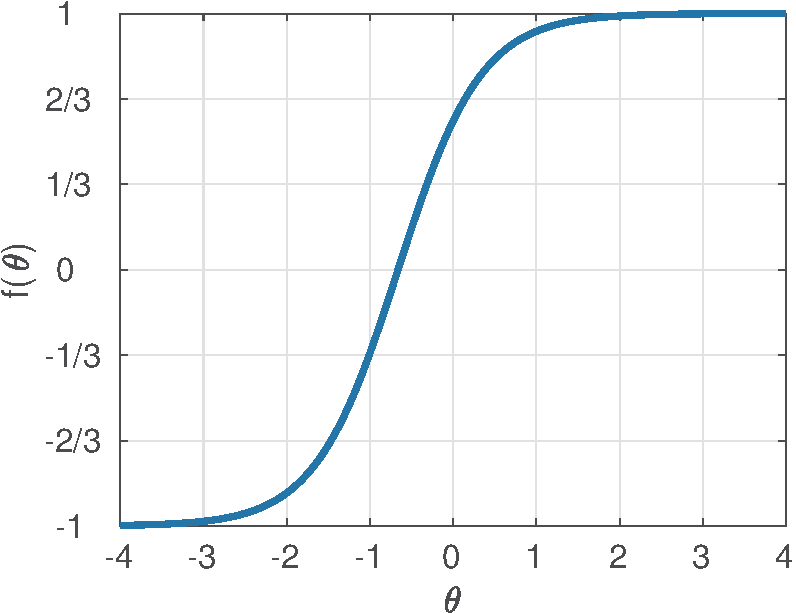
\includegraphics[width=0.4\textwidth]{Ising-MLE}
\end{center}

  \begin{solution}

    Denoting the $i$-th observed data point by $(x_1^i,x_2^i)$,
    the log-likelihood is
    \begin{align}
      \ell(\theta) & = \sum_{i=1}^n \log p(x_1^i,x_2^i; \theta)
    \end{align}
    Inserting the definition of the $p(x_1,x_2;\theta)$ yields
    \begin{align}
      \ell(\theta)  & = \sum_{i=1}^n \left[ \theta x_1^i x_2^i+x_1^i+x_2^i \right] - n \log Z(\theta)\\
      &= \theta \sum_{i=1}^n \left[x_1^i x_2^i\right] + \sum_{i=1}^n \left[x_1^i+x_2^i \right] - n\log Z(\theta)
    \end{align}
    Its derivative with respect to the $\theta$ is
    \begin{align}
      \frac{\partial \ell(\theta)}{\partial \theta} & =  \sum_{i=1}^n \left[x_1^i x_2^i\right] - n  \frac{\partial \log Z(\theta)}{\partial \theta}\\
      & =  \sum_{i=1}^n \left[x_1^i x_2^i\right] - n f(\theta)
    \end{align}
    Setting it to zero yields
    \begin{align}
      \frac{1}{n}  \sum_{i=1}^n \left[x_1^i x_2^i\right] &= f(\theta)
    \end{align}

    An alternative approach is to start with the more general
    relationship that relates the gradient of the partition function
    to the gradient of the log unnormalised model. For example, if
    $$ p(\x,\thetab) = \frac{\phi(\x; \thetab)}{Z(\thetab)}$$
    we have
    \begin{align}
      \ell(\thetab) &= \sum_{i=1}^n \log p(\x_i;\thetab) \\
      & = \sum_{i=1}^n \log \phi(\x_i;\thetab) -n \log Z(\thetab)
    \end{align}
    Setting the derivative to zero gives,
    $$\frac{1}{n} \sum_{i=1}^n \nabla_{\thetab}  \log \phi(\x_i;\thetab) = \nabla_{\thetab} \log Z(\thetab)$$
      
    In either case, numerical evaluation of  $1/n \sum_{i=1}^n x_1^i x_2^i$ gives
    \begin{align}
      \frac{1}{n}  \sum_{i=1}^n \left[x_1^i x_2^i\right] & = \frac{1}{3}\left(1-1-1\right)\\
      &= -\frac{1}{3}
    \end{align}
    From the graph, we see that $f(\theta)$ takes on the value $-1/3$
    for $\theta = -1$, which is the desired MLE. 

  \end{solution}

\end{exenumerate}

\ex{Parameter estimation for unnormalised models}
Let $p(\x; \A) \propto \exp(-\x^\top \A \x)$ be a parametric
statistical model for $\x = (x_1, \ldots, x_{100})$, where the
parameters are the elements of the matrix $\A$. Assume that $\A$ is
symmetric and positive semi-definite, i.e.\ $\A$ satisfies $\x^\top
\A \x \ge 0$ for all values of $\x$.

\begin{exenumerate}
\item For $n$ iid data points $\x_1, \ldots, \x_n$, a friend
  proposes to estimate $\A$ by maximising $J(\A)$,
  \begin{equation}
    J(\A) = \prod_{k=1}^n \exp\left( - \x_k^\top \A \x_k \right).
  \end{equation}
  Explain why this procedure cannot give reasonable parameter estimates. 

  \begin{solution}
    We have that $\x_k^\top \A \x_k \ge 0$ so that $\exp\left( -
    \x_k^\top \A \x_k \right) \le 1$. Hence $\exp\left( - \x_k^\top \A
    \x_k \right)$ is maximal if the elements of $\A$ are zero. This
    means that $J(\A)$ is maximal if $\A = 0$ whatever the observed
    data, which does not correspond to a meaningful estimation
    procedure (estimator).
    
  \end{solution}
  
\item Explain why maximum likelihood estimation is easy when the $x_i$
  are real numbers, i.e. $x_i \in \mathbb{R}$, while typically very
  difficult when the $x_i$ are binary, i.e.\ $x_i \in \{0,1\}$.

  \begin{solution}

    For maximum likelihood estimation, we needed to normalise the
    model by computing the partition function $Z(\thetab)$, which is
    defined as the sum/integral of $\exp(-\x^\top \A \x)$ over the
    domain of $\x$.

    When the $x_i$ are numbers, we can here obtain an analytical
    expression for $Z(\thetab)$.  However, if the $x_i$ are binary, no
    such analytical expression is available and computing $Z(\thetab)$
    is then very costly.
    
  \end{solution}
  
\item Can we use score matching instead of maximum likelihood
  estimation to learn $\A$ if the $x_i$ are binary?
  
  \begin{solution}
    No, score matching cannot be used for binary data.
  \end{solution}
  
  
\end{exenumerate}

